\documentclass[twoside]{article}
\usepackage[utf8]{inputenc}
\usepackage{amsmath,amsfonts,amssymb,amsthm,latexsym}
\usepackage[spanish,es-noshorthands]{babel}
\usepackage[T1]{fontenc}
\usepackage{lmodern}
\usepackage{graphicx,hyperref}
\usepackage{tikz,pgf}
\usepackage{marvosym}
\usepackage{multicol}
\usepackage{fancyhdr}
\usepackage[papersize={5.5in,8.5in},left=.75cm,right=.75cm,top=1.5cm,bottom=1.25cm]{geometry}
\usepackage{fancyhdr}
\pagestyle{fancy}
\fancyhead[LE]{\Email iedabgerman@autistici.org}
\fancyhead[RE]{}
\fancyhead[RO]{\url{https://www.autistici.org/mathgerman}}
\fancyhead[LO]{}

\author{Germ\'an Avenda\~no Ram\'irez~\thanks{Lic. Mat. U.D., M.Sc. U.N.}}
\title{\begin{minipage}{.2\textwidth}

\includegraphics[height=1.75cm]{Images/logo-colegio.png}\end{minipage}
\begin{minipage}{.55\textwidth}
\begin{center}
Taller 2\\
Números naturales $\mathbb{N}$\\
Aritmética $6^{\circ}$
\end{center}
\end{minipage}\hfill
\begin{minipage}{.2\textwidth}

\includegraphics[height=1.75cm]{Images/logo-sed.png} 
\end{minipage}}
\date{}
\thispagestyle{plain}
\begin{document}
\maketitle
\begin{minipage}{.95\textwidth}
\fbox{\textit{No raye ni dañe esta hoja para que pueda usarla otro compañero}}
\end{minipage}
\section*{Continuación taller 1}
\subsection*{Nivel II}
\begin{enumerate}
\item Redondea el valor de los términos de las siguientes operaciones y estima el valor de sus resultados. (Por ejemplo para multiplicar $3258\times 22$, multiplicamos $3260\times 20$ con lo cual obtenemos $65200$, el cual es un valor aproximado de la multiplicación $3258\times 22$)
\begin{enumerate}
\begin{multicols}{2}
\item $4978+5235+3102$
\item $6789-1986$
\item $342\cdot 56$
\item $4986\div 56$
\end{multicols}
\end{enumerate}
\item La diferencia entre dos números es 1.284 y el mayor es igual al triple del menor. ¿Cuáles son los números?
\item En una librería se han vendido hoy 315 libros más que ayer. Entre los dos días se vendieron 1325 libros. ¿Cuántos se han vendido cada día?
\item Al multiplicar un número por 24, su valor aumenta en 1.334 unidades. ¿Cuál es el número?
\item Laura hace ramos de flores. Si coloca 12 flores en cada ramo le salen 8 ramos y le sobran algunas flores. Si tuviera 8 flores más, podría hacer 9 ramos y no le sobraría ninguna flor. ¿Cuántas flores tiene Laura?
\item ¿Cuál es el número que al dividirlo entre 43 su cociente es igual a 34 y el resto toma el mayor valor posible.
\item Mi madre lava 1 camisa y cuesta secarse 1 hora y media y un vaquero cuesta secarse 2 horas. ¿Cuánto tardarán en secarse dos camisas y dos vaqueros tendidos a la vez?
\end{enumerate}
\subsection*{Nivel III}
\begin{enumerate}
\item Explica la propiedad distributiva de la multiplicación respecto a la suma y resuelve de dos maneras los siguientes productos:
\begin{enumerate}
\begin{multicols}{2}
\item $17\cdot 38+17\cdot 12$
\item $96\cdot 59+4\cdot 59$
\item $149\cdot 19+52\cdot 19$
\end{multicols}
\end{enumerate}
\item Saca el factor común en las siguientes expresiones:
\begin{enumerate}
\begin{multicols}{2}
\item $7\cdot 5-3\cdot 5+16\cdot 5-5\cdot 4=$
\item $6\cdot 4-4\cdot 3+4\cdot 9-5\cdot 4=$
\end{multicols}
\end{enumerate}
\item Saca el factor común en las siguientes expresiones: (Por ejemplo $50+150-25$ tiene como máximo factor común a $25$, ya que \[50+150-25=2(25)+6(25)-1(25)\] por tanto al sacar el factor común se obtiene \[25\cdot[2+6-1]=25\cdot [7]=175\]
\begin{enumerate}
\begin{multicols}{2}
\item $120+130+170=$
\item $25+35+50=$
\item $48-16+72$
\end{multicols}
\end{enumerate}
\begin{enumerate}
\item Resuelve y comprueba (Recuerde que $4^{3}=4\cdot 4\cdot 4=64$)
\begin{multicols}{3}
\item $(3^{4})^{4}=$
\item $(8^{2})^{3}=$
\item $(9^{3})^{2}=$
\end{multicols}
\end{enumerate}
\item Calcule la raíz cuadrada de los siguientes números (para calcular la raíz cuadrada de un número como $144$, se descompone éste en sus factores primos así: $144=2^{4}\cdot 3^{4}$, luego para extraer raíz cuadrada, usamos la propiedad distributiva de la radicación respecto a la multiplicación:
\[\sqrt{144}=\sqrt{2^{4}\cdot 3^{4}}=\sqrt{2^{4}}\cdot \sqrt{3^{4}}=2^{2}\cdot 3^{2}=4\cdot 3=12\]
\begin{enumerate}
\begin{multicols}{2}
\item $7'342.987$
\item $16'920.000=$
\end{multicols}
\end{enumerate}
\item Realice las siguientes operaciones:
\begin{enumerate}
\begin{multicols}{2}
\item $3+6\cdot 5-3\cdot 4-2=$
\item $3+(6+4)\cdot 5-4\cdot 6-3+(2\cdot 8)\div 4=$
\item $7\cdot 3+[6+2\cdot (8\div 4+3\cdot 2)-7\cdot 2]+9\div 3=$
\end{multicols}
\end{enumerate}
\item La suma de dos números es 288 y el cociente entre ellos es 8. ¿Cuáles son los números?
\item Don Tomás quiere repartir unos libros entre sus hijos. Puede hacerlo dándoles 1 al mayor, 2 al segundo, 3 al tercero \ldots Otro modo de repartirlos sería dar 7 a cada uno. ¿Cuántos hijos y cuántos libros tiene Don Tomás?
\item El producto de dos números es 64 y su suma 20. ¿Cuáles son esos números?
\item Se reparten 9.000 pesetas\footnote{Moneda usada en España} entre 4 amigos de manera que: el segundo reciba el doble que el primero; el tercero triple que el segundo; y el cuarto reciba lo mismo que los otros tres juntos. ¿Cuánto recibe cada uno?
\item ¿Cuál es el menor número que cumple estas condiciones: al dividirlo entre 4 el resto es 3; al dividirlo entre 5 el resto es 2 y al dividirlo entre 7 el resto es 3.
\item Maite quiere comprar sellos. Tiene menos de 100 pesetas, si los compra todos de 5 pesetas, le sobra una peseta. Si los compra de 8 pesetas le sobran 6 pesetas. Le falta una peseta para comprar un número exacto de sellos de 29 pesetas. ¿Cuánto dinero tiene Maite?
\item Entre Ramiro y Raúl tienen 1.255 pesetas. Entre Ramiro y Rita tienen 1.305. Entre Rita y Raúl tienen1.390. ¿Cuánto dinero tiene cada uno?
\item En una granja se han vendido 1482 huevos. Si dos docenas y media cuestan 540 pesetas, ¿Cuánto valen los huevos?
\item Un camionero carga en su camión 4 televisores y tres microondas. Si cada televisor pesa como tres microondas y en total ha cargado 75 kilos ¿Cuánto pesa cada aparato?
\item Cada gallina de una granja pone dos huevos en tres días. ¿Cuántos días tardarán cuatro gallinas en poner tres docenas de huevos?
\item Las edades de un padre y su hijo suman 100 años. Cuando el padre tenía la edad que hoy tiene el hijo, sus edades sumaban 56 años. ¿Cuál es la edad de cada uno?
\item Un padre le saca a su hijo 25 años. Dentro de dos años el padre tendrá el doble de edad que el hijo. ¿Cuántos años tiene cada uno en la actualidad? 
\item ¿Cuántas chocolatinas de 60 gramos hay en una docena y media? 
\item ¿Cuántos metros de tela a cuadros se pueden comprar con dos billetes de 1.000 pesetas, una moneda de 500 pesetas y 6 monedas de 25 pesetas, si la pieza de tela mide 50 metros?
\item Si un ladrillo pesa 2 kilos y medio ladrillo. ¿Cuánto pesa ladrillo y medio?
\end{enumerate}
\subsection*{Problemas}
\begin{enumerate}
\item Si \begin{tikzpicture}
 \draw (-1,0) rectangle node {a} (0,1);
 \draw (0,0) rectangle node {b} (1,1);
 \draw (-.5,1) rectangle node {$a+b$} (.5,2);
\end{tikzpicture}
complete mentalmente la pirámide
\begin{tikzpicture}
\draw (-2,0) rectangle (-1,1);
\draw (-1,0) rectangle (0,1);
\draw (0,0) rectangle node {2}(1,1);
\draw (1,0) rectangle (2,1);
\draw (-1.5,1) rectangle (-.5,2);
\draw (-.5,1) rectangle node {6}(.5,2);
\draw (.5,1) rectangle (1.5,2);
\draw (-1,2) rectangle node {16}(0,3);
\draw (0,2) rectangle (1,3);
\draw (-.5,3) rectangle node{29} (.5,4);
\end{tikzpicture}
\item ¿Cuántos números de tres dígitos diferentes tienen suma digital 22?
\item Halle el valor numérico de cada uno de los símbolos
\begin{align*}
\square + 8 &=\lozenge & \square=?\\
\lozenge \div 5&=\bigcirc &\lozenge=?\\
\bigcirc \cdot 7&=\star & \bigcirc =? \\
\star -10&=11 & \star=?
\end{align*}
\item ¿Cuántos cuadrados hay?
\begin{tikzpicture}
\draw (0,0) grid (4,2);
\end{tikzpicture}
\item ¿De cuántas maneras diferentes puede cambiarse un billete de \$1000 y de \$2000?
\item Si $A$ y $B$ con consecutivos, halla $A$, $B$ y $C$
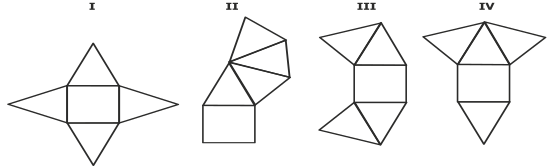
\includegraphics[scale=.35]{Images/Pantallazo.png} 

\begin{minipage}{.5\textwidth}
\item Distribuye los dígitos 1, 2, 3, 4, 5 y 7 en los 7 círculos de la figura de tal manera que en cada segmento de tres círculos se cumpla: El doble del dígito del centro es igual a la suma de los números extremos.
\end{minipage}
\begin{minipage}{.45\textwidth}
\begin{tikzpicture}
\draw (0,0) circle (10pt) node  (a){};
\draw (2,0) circle (10pt) node (b){};
\draw (4,0) circle (10pt) node (c){};
\draw (1,2) circle (10pt) node (d){};
\draw (3,2) circle (10pt) node (e){};
\draw (2,4) circle (10pt) node (f){};
\draw (a) -- (b);
\draw (b) -- (c);
\draw (c) -- (e);
\draw (e) -- (f);
\draw (f) -- (d);
\draw (d)--(a);
\end{tikzpicture}
\end{minipage}
\end{enumerate}
\end{document}
